\begin{center}
An ontology-based retrieval system using semantic indexing

基于本体的语义检索系统
\end{center}
\renewcommand{\thetable}{\arabic{table}}
\renewcommand{\thefigure}{\arabic{figure}}
\setcounter{figure}{0}
\setcounter{table}{0}
\xiaosihao
\setlength\parindent{2em}
\setlength{\baselineskip}{20pt} %设置行间距17pt
\renewcommand\refname{参考文献}

摘要

在这篇文章里,我们展现了一种基于本体的信息抽取和检索系统,以及它在足球领域的运用。总的来说,我们解决了在语义搜索中的三个问题,也就是,使用性,可扩展性和检索效果。我们提出了一种基于关键词的语义检索方法。使用具体领域的信息抽取之后,系统性能得到了显著的提升。通过语义索引方法以及用一个小的独立模型来代表世界,可扩展性也得到了实现。系统用全世界最先进语义网技术来实施,其性能可与传统方法和扩展查找法相媲美。此外,我们还提出了一种具体的评价指标,来观测专门领域的信息抽取与推理的性能表现。最后,我们展示了我们是如何采用语义检索的方法来解决简单的结构性二义性的。

1.导言

互联网上可获得信息的数量与复杂性都在爆炸性增长,人们就迫切需要一种工具和技术来通过语义地掌握这些数据。现在的信息检索方法主要基于搜索全文的关键字,也就是一个海量词包的模型。然后,这样的模型丢失了很多真正的文本语义信息。为了解决这个问题,本体技术,作为一种知识表达的方式就应运而生,它也成为了当今语义网应用的支柱。能够给普通文本赋予语义的元数据,也就为信息抽取和检索过程提供了极大的便利。

当语义知识通过本体表达出来,下一步就是要查询语义数据,也就是语义搜索。现在有几种用于语义查询的查询语言。现在,{\Times SPARQL}是语义网最先进的查询语言。但不巧的是,这些正式的查询语言并不能很好地被末端用户使用。用这些语言严谨描述一个查询需要领域本体和语言的语法。因此,语义网研究团体为末端用户简化检索过程。当下的语义检索接口研究主要包含了四种类型:基于关键词的,基于形式的,基于视觉的,基于自然语言的。其中,基于关键词是操作最友好的,人们也习惯于使用这种接口,在这个问题上,幸亏有谷歌搜索。

在语义搜索领域,能够整合关键词方法的易用性和语义技术的强大性,是极具挑战性的技术。根据我们对语义网的观察,所有对保证用户友好层的基础上提高检索性能的努力都会带来这样的结果,那就是改善采用关键词接口的语义搜索。这是一项极具挑战性的任务,因为它需要用简单的关键词完成复杂的检索。此外,它还要求能够使推理信息得以被轻易检索,并且提供一种排序机制反映语义和本体的重要性。

在本文中,我们展示了一种完全基于本体的框架来实现对特定领域的语义信息的抽取和检索。这个系统含有爬虫模块,自动的信息提取模块,本体运用模块,推理模块,和关键词语义搜索的界面。我们主要考虑的是创造一种可扩展的、用户友谊好的、检索性能优异的检索系统。我们把这个框架运用在了足球领域,并且看到了相对于传统的关键词搜索的显著提高。我们展示了我们系统对于足球领域非常复杂的查询也实现了极高的查准率和查全率。此外,我们评估并报告了依照语义性过程(只采用信息抽取和同时采用信息抽取和推理)在不同程度的索引方法下的查询效果。

可扩展性被分为两个主要方面来考虑:推理和查询。在推理方面,可扩展性要求把完全的逻辑模型拆分成单独的独立模型,因为在一个大模型下搜索比在一堆小模型下搜索要复杂很多。一些相似的研究也着眼于用一个模型来描述整个世界。因此,他们并不能匹配大尺度的。

在查询方面,可扩展性要靠把推理的知识转化成一个单独的逆索引结构来保证。用这种逆索引结构可以把我们的系统向上扩展到网页搜索引擎,也就意味着可以在较短时间内完成几百万个搜索,并且从少量的数据中检索出想要的信息。它也触发了关键词搜索的使用。用这种方法,就可以支持用户友好的查询方式。基于信息检索的本体研究采用本体模型中的逻辑查询。因此,相比于网络尺度来说,它只能被用在较少量的数据搜索中,而且对于普通用户来说,逻辑搜索也是一个困难的工作。

文章的剩余部分按照如下思路组织:在第二部分简要讨论相关的研究工作成果,在第三部分系统的主要组成部分,也就是信息抽取,本体构建、推理和信息检索。在第四部分,我们给出了评估结果。第五部分给出与扩展搜索方法的简单比较。第六部分阐释了系统支持短语描述扩展的机理。第七部分,我们进行简单的讨论,在第八部分,总结全文,并对未来工作进行展望。

2.相关研究

经典的,或者说传统的基于关键词的信息检索方法是基于{\Times Salton}等人提出的向量空间模型。在这种模型中,文本和查询都是被简单的表述关键词术语权值向量,检索就根据这些向量的余弦相似度来完成。与传统搜索相关的重要工作在文献4~7中描述。这种方法不需要任何抽取或者是注释语句,因此它更容易实施,然而,查准率相对较低。向量空间在现实生活中的运用,是采用了诸如{\Times Lucene}的逆索引结构来实现的。换句话说,{\Times Lucene}类似的工具建立了向量空间模型的理论背景和现实世界应用的联系。

语义检索的第一部是要利用词汇网络的同义词表解决单词语义。其主要思想是利用单词的主义来同时扩展目录和查询,以期更好的查准率和查全率。如果同时采用了有效的词感模糊算法({\Times WSD}),这种方法提升了检索性能。从另一方面说,一个不好的WSD将会导致性能下降。这种方法的另一个缺点是缺乏复杂主义,因为他被局限在了词汇网络的有限关系中。

语义检索的下一步是采用信息抽取。有很多这个领域的研究。他们主要的区别在于资源的结构,抽取信息的细节和计算/记忆资源。基于{\Times NLP}的方法是独立的,因为使用了句子的解析树,自动词性赋码器,数据块解析,首语重复解决方法等,以期能够抽取信息。他们都需要大量的计算过程。也有一些信息抽取方法的选择,比如基于特征/规则的信息抽取就不用特别庞大的计算开销。这些方法根据特征/规则的创建形式来分类:自动,手动。如果考虑在某一个领域付出的劳动的话,相比于手动法,自动法显得更高级,但其查准率查全率又不理想。

文献22~26使用的方法是采用人工建立的规则来抽取信息。人工建立规则也被用于语义性的注释。{\Times Etztioni}等人用独立的规则来定位文本中不同类型的个体。{\Times Wessman}等人主要依靠常规表述。{\Times Cerno}是一个用于领域本体描述语义性注释和文本文档的轻量级框架。它整合了基于关键词和基于结构的注释规则,而不是语言学的特征。我们需要一种可扩展的,应对刚性结构化领域的信息抽取方法。这种方法应该也能被用于土耳其语和英语内容。由于抽取信息的细节对我们的目标非常关键,我们必须非常关注查全率和查准率直。因此我们采用了手动填加的方法,因为在其中,技术细节已经被给出了。

关于本体设计、集成和重组的研究提供了很多基于本体的信息抽取和检索方法。{\Times Oberle}等人提出了一种基本的本体,{\Times SmartSUMO},它是基于{\Times DOLCE}和 {\Times SUMO} 本体的,其目的是集成用于智能网络的领域本体,最后的集成本体被称为智能网络集成本体({\Times SWIntO})。因为 {\Times SmartSUMO}同时具有语言学特性,{\Times SWIntO}被用在基于本体的文本信息抽取。也一种面向本体设计的固定方法。文本信息用一种健全的方法被映射成为本体概念。然而,整个集成本体在遇到一个新的语言结构就会受到影响,因为语言性特征就是基础本体的一部分。为了避免这种困难,词汇特性要被独立于基础本体和领域本体来考虑。我们选择的本体设计并不考虑基础本体,因为我们暂时还没有针对不同领域的集成目标。然而,我们通过一种把词汇特性映射到本体的信息抽取方法,保留了词汇信息独立于本体的思路。就基于本体的信息检索系统的各个方面问题,现在都进行了很多讨论。文献34的基于本体的信息检索研究,主要着眼于让{\Times MPEG7/21}标准与领域和应用本体之间能够彼此协作。在我们的研究中,我们开发了一个中心足球本体,它可以表现出足球领域的知识。我们的本体被认为与文献34中的足球本体在独立于互用性的领域知识方面一样强大。另一方面,文献34中提出的检索方法是严格的。因为检索方法都是基于逻辑查询的,建立搜索查询对于一般的用户来说是极困难的。在这个条件下,我们提出了一种基于查询结果方法的索引,使用户可以用一种简单灵活的方法来查询基于本体的知识。

文献35讨论了本体用于在组织记忆中进行信息检索,探究了组织化,访问性,保存大量异相信息的元级描述的重要性。也有研究提了了有理解力的元级模型和检索的基于本体的方法。本体可以分为几类:领域本体,信息本体,企业本体等。他们都采用一种常规的面向对象的形式进行建模。根据这个分类,我们用领域本体来代表足球比赛,这个领域本体被用于推理那些从比赛总结中没有精确提取的信息。在我们的研究中,没有明确的搜索。我们都用逆索引来重构推断的信息,并提供查询结果。

在一个信息检索系统中,用于查询本体知识的用户界面是至关重要的一个点。通用的方法是把解析出的数据以{\Times RDF}或{\Times OWL}的形式存储起来,再用{\Times RDQL}或 {\Times SPARQL}等查询语言云查询{\Times RDF}。尽管这种方法有极好的查准率和查全率,它还是不能用于实用,因为它需要相对复杂的查询语言。为了克服学习一种正式查询语言的困难,现在又提出了很多查询页面的方法。正如我们早些所说,我们主要的重要应该放在的有几种方法在基于关键词的界面。目前有几种方法是实施了基于关键词的搜索的。简单地说一说,{\Times SPARK}用了概率查询排序法来找出关键词所代表的最佳查询。{\Times Q2}语义尽力在一个{\Times RDF}图中找到代表查询的最佳子图。{\Times SemSearch}用了一种基于模板的方法来进行查询。这些方法都不容易被扩大到大量知识的情况,因为他们都需要{\Times RDF}图或是为了一次搜索要对同样的基础知识进行多次查询。

一种可扩展的从关键词进行查询构建的选择是语义索引。在这种方法中,{\Times RDF} 基础知识中的语义数据被用一种结构化的方法索引,并且能直接为关键词查询所用。一种相似的方法被用在了文献40~42中。他们为所以{\Times RDF}中解析出来的三元组和相关的自由文本做了索引。因为他们采用了非常基础的的提取方法,这样一种简单的索引看起来是可行的。然而,从只包含了主谓宾的索引中并不能提取出复杂语义。如果要求系统能够从解析和推理的知识中完成复杂查询,那么索引就必须被进行相应的设计和充实。在文献43中,展示了一种基于多模式通用语义网搜索接口,以及其在2006足球世界杯中数据的运用。重点在于形成一种回答问题的系统,它能够考虑到基于与用户交互的论述和上下文的信息,并且以语义网为基础形成一个语义查询。据记录,对于某些查询,这个过程的次数上升到最小2次。考虑到查询与文献43所提到的足球相关,我们的系统不仅成功地控制了所有的数据,而且通过利用语义索引实现了即时查询,强调了可扩展性和性能表现等问题。此外,我们的本体个体是通过网络描述的信息自动抽取出来进行构建的,然后再基于推理应用规则使其充实。

我们的文献调研提示了当前基于关键词语义搜索的研究是不够成熟的:他们即不能扩展到大尺度的基础知识,也不能在查询中捕获所有的语义。我们的主要贡献是通过实施一种基于关键词的使用语义索引方法的语义检索系统,填补了这方面的空白。换句话说,我们尽量的实施这样一种系统,其表现至少与传统方法一样好,能够在性能和语义查询的实用性上有所提高。我们在足球领域检测我们的系统,看看传统搜索方式之上的语义搜索的有效性,我们观测到了查准率和查全率上可喜的提高。我们注意到我们的系统可以完成复杂语义的查询,而传统方法是不可能做到的。本文所展示的方法可以通过修改现行的本体和文献30所述的信息提取方式,被扩展到其他领域。

3.我们语义检索的方法

在本文范围内,我们开发了一种完全成熟的语义应用,它包含了从信息提取到信息检索的语义网的各个方面,并且使用了所有的分词技术,比如{\Times OWL-DL},推理,规则,{\Times RDF}库和语义索引。框架的全部图解如图一所示。后面的部分以对全对程的简单总结开始,描述了系统的几个重要方面。

	\begin{figure}[htbp] 
	\centering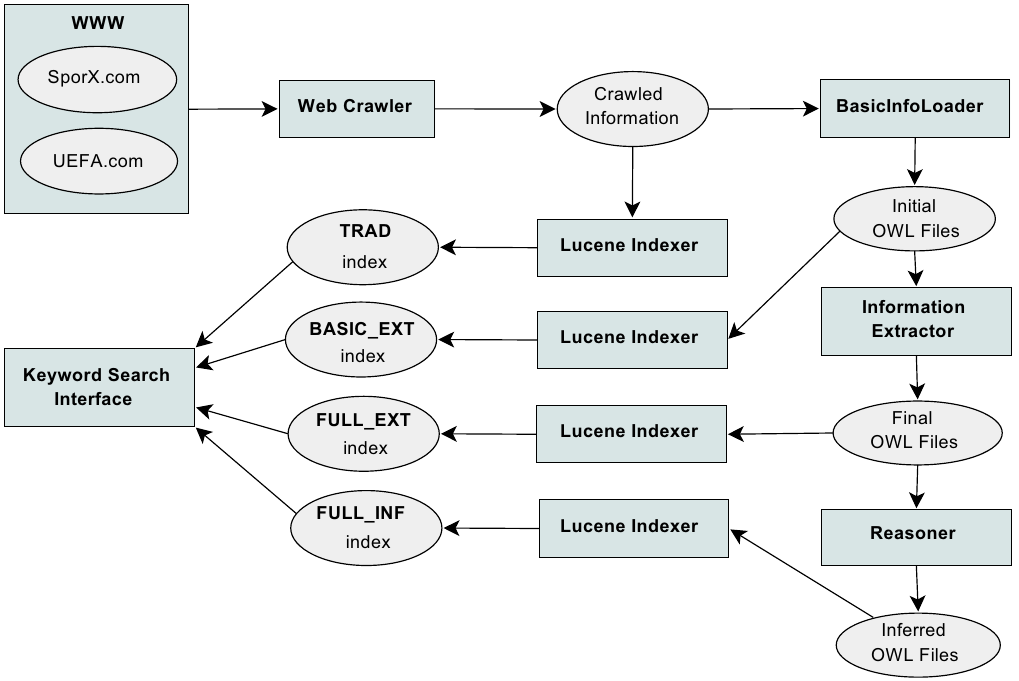
\includegraphics[width=5in]{fig/trans/fig1.png} 
	\caption[]{\xiaosihao 系统框架图}
	\end{figure} 
3.1全过程

在给出各模块的技术细节之前,我们认为先来看看我们用于足球领域的系统的全工作流会很有帮助。接下来,我们描述在系统准备好进行语义查询和评估之前的步骤。

{\Times a}.通过爬虫在{\Times UEFA}和{\Times SporX}等网站上获得有用信息,并临时性地存储起来。所得数据包括了一些基本信息,比如队伍、队员、进球、替补、每场球赛的场馆,以及以自由文本形式工出现的按时间的解说。

{\Times b}.只用自由文本的解说来建立索引,{\Times TRAD},以进行传统的关键词搜索。

{\Times c}.用这些基本信息和解说,我们建立了原始的{\Times OWL}文件。

{\Times d}.通过这些原始{\Times OWL}文件,我们建立第二个索引,{\Times BASIC\_EXT},它包含了基本信息和解说。这个索引只是为了评估而建立(也就是说,用它和索引{\Times FULL\_EXT} 进行比较,后者是在信息抽取之后建立的)。 

{\Times e}.上一步建立的{\Times OWL}文件通过信息抽取模块读取。这个模块建立了具有从解说中提取出来的信息的{\Times OWL}文件,信息包括越位,犯规,角球等,以此来获得最终的{\Times OWL}文件。

{\Times f}.读取并索引这些{\Times OWL}文件,从而建立{\Times FULL\_EXT}。

{\Times g}.我们对这些文件运行了推理机,获得了一个新的包含推理信息的新的{\Times OWL}文件

{\Times i}.最后,我们用这些推理的{\Times OWL}文件建立一个索引,{\Times FULL\_INF},也就是最后一个用于语义搜索的索引。

尽管我们在研究中只着眼于足球领域,但是上述方法可被运用到其他有给出本体的领域。这个系统最针对某个领域的模块是{\Times IE}模块,它应该被扩展来解决其他领域的问题。文章的剩下部分描述了系统的几个主要组件。我们以建立领域本体开始,然后是{\Times IE}和{\Times IR}组件,最后我们来看看评估结果。

3.2本体设计

本体是概念和概念之间关系的一种描述。他们通过提供真实世界对角的共用知识,在语义网络应用中扮演重要角色,它也有效提升了重用性和不同模块之间的互换性。因此,本体的质量是任何语义应用的首要考虑的问题。

对于这项研究,我们设计了一个中心足球本体,它利用了这个系统的各个方面,尤其是在信息抽取,推理和检索词组等方面。在本体设计阶段,我们遵循了一个迭代的过程。首先,我们以一个包含核心基本概念和一些简单分类的本体为起点。然后,我们用这个本体进行实验,解决了其在推理和搜索中的一些问题。这些步骤一直重复,直到我们得到了一个含有79个概念和95个属性的足球领域的稳定本体。完成的类树如图2所示。

	\begin{figure}[htbp] 
	\centering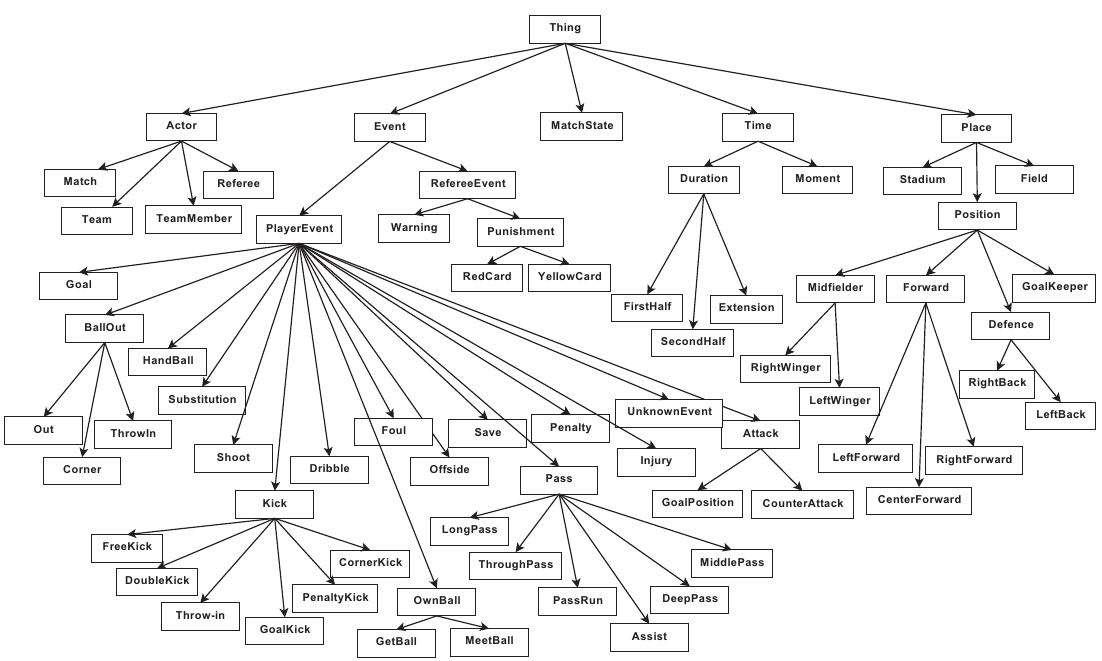
\includegraphics[width=5in]{fig/trans/fig2.png} 
	\caption[]{\xiaosihao 领域本体,类结构}
	\end{figure} 

3.3 信息抽取({\Times IE})

信息抽取是基于本体的语义网应用的重要组成部分。它是把非结构化的资源转化成结构化的信息,并存入信息基础的过程。在这个阶段,我们用爬虫从{\Times UEFA}和{\Times SporX}获得的数据。我们所获得的东西是一些具体到比赛(队伍,队员,进球,场馆等)的信息和一些自然文体(关于比赛的不断的解说)。这些基本信息和解说被用作信息抽取模块的输入。这个模块的技术细节在文献30中有描述。在研究中,我们只是从功能角度进行了概览。

基本上,这是一个基于模版针对具体领域的{\Times IE}方法。不像其他自动方法,它并不采用词性标签,语法剖析器和短语识别等语言性的工具。因此我们的方法可以被用在任何领域,任何语言,而不必彩语言工具,尽管人工建立模板是它的一大缺点。{\Times IE}模块的细节可以总结成了两个部分:命名实体识别器和词汇分析器。

3.3.1 命名实体识别器({\Times NER})

如之前所提到的那样,{\Times IE}模块把一些诸如队伍、队员的信息作为输入作为解说的补充。这些信息被用来识别和分类解说中的命名实体。通过运行{\Times NER},队伍名称和队员名称被{\Times <team1>},{\Times <team2>},{\Times <team1player5>}这样的标签所取代。例如,一个句子“{\Times Iniesta}得分”就可能变成“{\Times <team2player11>}得分”,如果{\Times Iniesta}是这只队伍的11号的话。

3.3.2 两个层次的词汇分析

这是我们{\Times IE}模块最关键的部分,在这儿,复杂的语义实体和关系都将根据预先定义的模板进行解析。第一个层次是要定义关键词/词组并且忽略剩余的部分。第二个层次是把第一层的输出作为该层的输入,并且根据预告定义的模板进行解析。根据我们的调查,大多数语义网的研究都缺乏这种类型的解析,因为他们通常对NER产生的注解就很满意了。

根据文献30所述,多亏了{\Times UEFA}网站的高度结构化文本和零错误,我们得以实现{\Times UEFA}解说的100%的成功率。图3给出了我们可以从{\Times UEFA}网站抽取信息的想法。这个模块与系统的集成采用了时下流行的松散耦和形式,所以我们能够把它用于任何语言任意领域的语义性应用中。

	\begin{figure}[htbp] 
	\centering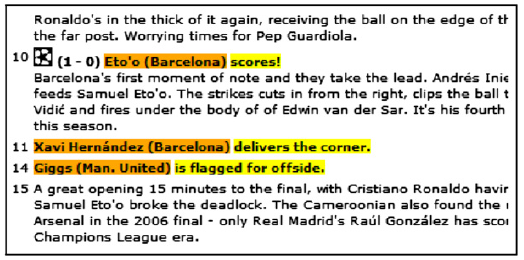
\includegraphics[width=3in]{fig/trans/fig3.png} 
	\caption[]{\xiaosihao {\Times UEFA}解说解析样例}
	\end{figure} 

3.4建立本体

建立本体的过程是要把非结构化、半结构化或结构化的数据转换或是映射成本体实例,以此获得知识。我们的信息抽取模块在把非结构化的文本解说解析成结构化的信息方面已经完成了大部分工作。例如,在解说词“{\Times Keita}在与{\Times Belletti}争抢时犯规“,我们就获得了一个犯规对像,更具体的说,就是{\Times FOUL (Keita, Belletti)}。

有了{\Times IE}模块的输出,建立本体的过程变成了为{\Times IE}所获数据的每个对象建立{\Times OWL} 实体。正是在这个阶段,{\Times IE}模块与系统的其他部分进行了集成。我们尽量让这种集成松散。通过定义高层的属性,我们解决了本体层折问题。一般情况下,本体里的每一个事件都有其一套属性。例如,根据一个事件的主语,一个犯规实例就有被罚球员这样一个属性,而一个进行实例就会有得分球员这样一个属性。问题在于通过{\Times IE}模块的信息来填补正确的属性值。我们对这个问题的解决方法是为本体中的每个事件定义四个一般属性,{\Times subjectPlayer}, {\Times objectPlayer}, {\Times subjectTeam}和 {\Times objectTeam}。这些属性都是一般的,针对每个事件还有具体的子类属性。例如进球事件就具有属性得分球员,它恰是 {\Times subjectPlayer}的一个字类属性。用这样的方法我们可以自动的通过这个事件的发出者,在得分事件中填补进球事件。相似地在受伤事件中受伤队员属性,就会被填以这个事件的客体,因为受伤队员属性在本体中被定义成了{\Times objectPlayer}的子类属性。

如果{\Times IE}模块不能解析一个事件中的任何一个属性, 我们可以创建一个有空属性的实例。因此,哪怕{\Times IE}没有能解析出事件的一些属性,对于简单查询查全率也不会受影响。此外,如果解说中没有提及事件,一个具有未知事件的实例也会被创建。未知事件并没有丢失,原因见如图4所示的起始于{\Times UEFA}解说、终止于{\Times OWL}实例的过程之描述。

	\begin{figure}[htbp] 
	\centering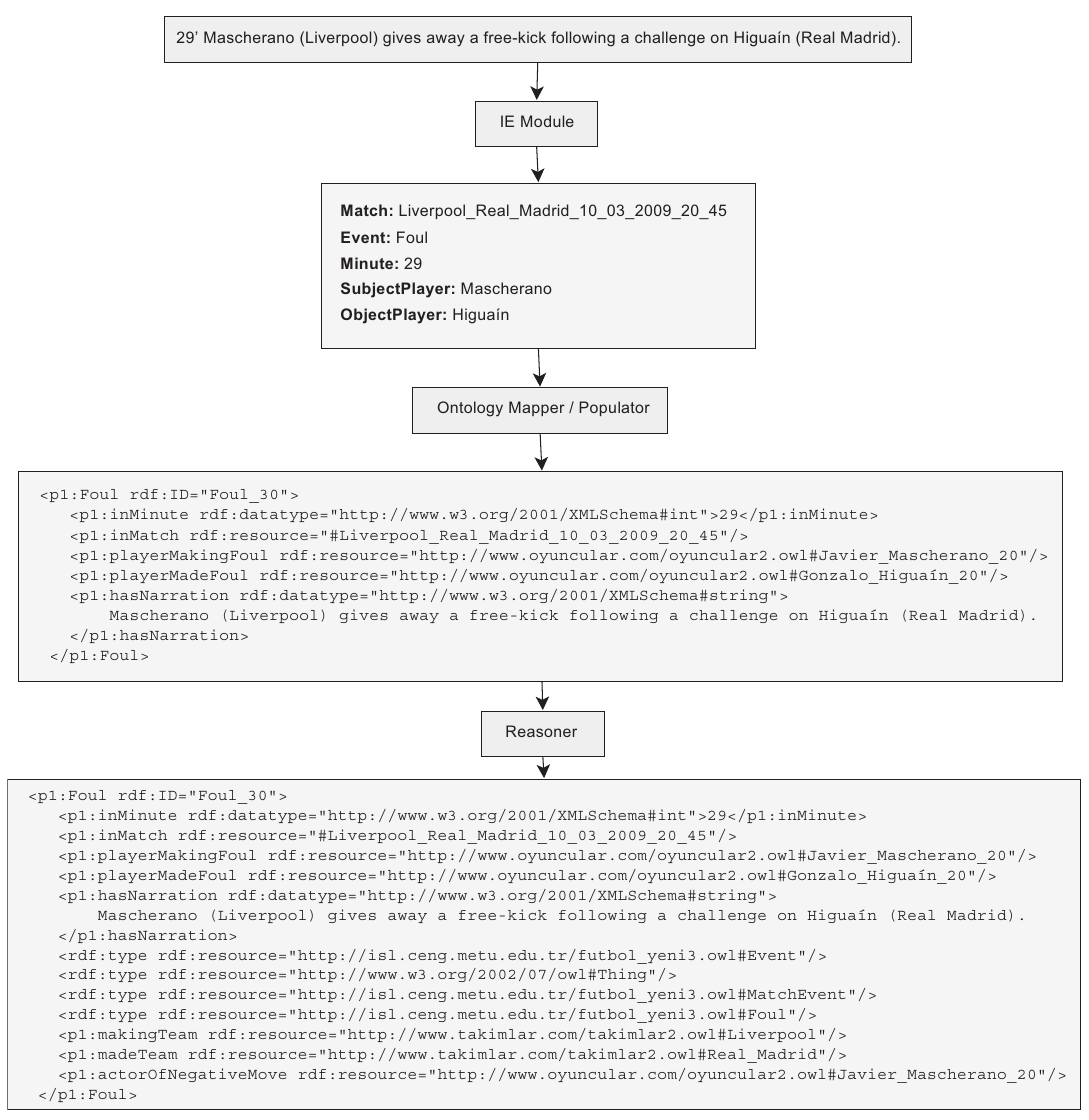
\includegraphics[width=6in]{fig/trans/fig4.png} 
	\caption[]{\xiaosihao 信息获取和本体化}
	\end{figure} 

用{\Times IE}模块解析事件进行本体建立并不严格,如之前所谘的,爬虫数据包含了关于比赛的基本基本信息,包括队员,队伍,裁判,场地等,这些信息如果在基础知识中不存在,则通过建立{\Times OWL}实体逐个填加到文本中。

3.5推理和规则

网页本体语言,{\Times OWL},是一个正式的标准,它很大程序上被描述逻辑({\Times DLs})影响着。{\Times OWL DL}是由计算机完成的,{\Times OWL}的可决定版本,它得益于有很多可靠完整{\Times DL}推理机。对于我们的推理模型,我们用了{\Times Pellet},一种开源的{\Times DL}推理机,它支持各种标准的推理服务,比如相容性检查,概念可满足性,分类,实现。

相容性检查保证了本体中没有相矛盾的声明。为了利用这种特性,我们在本体构建过程中细化了一些属性的约束条件。{\Times OWL}中有两种约束条件:值约束和集约束。我们用了值约束,比如,要陈述只有守门员(队员的子集)才被允许待在守门位置,然后用集约束,我们可以说一场比赛只允许有一个守门员。这些约束条件不仅在相容性检查中发挥作用,而且使得新信息可以被推断出来。例如,当某个实例的某个属性值的定义域被限制在一个特定的类,那我们可以推断出这个实例的类型了。

采用分类推理,我们可以根据本体中的类和子类的定义得到完整的类树。通过分类来推断新知识是独立于领域的过程,并且它对基础知识的影响是小的。如图5所示是一个简单的例子,长传的类树结构就是被推断出来的。

	\begin{figure}[htbp] 
	\centering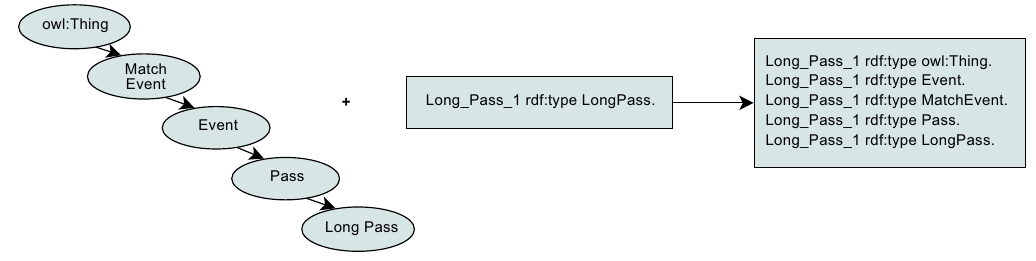
\includegraphics[width=6in]{fig/trans/fig5.png} 
	\caption[]{\xiaosihao 常传的类层次推理}
	\end{figure} 

为了推理更多的有意思的信息,我们用了{\Times Jena}规则。为了证明{\Times Jena}规则的强大之处,我们给出一个推理助功事件的例子。采用如图六所示的{\Times Jena}规则,我们能够在基础知识中增加一个助攻实例。这个规则只是找两个事件,一个是得分一个是发生在同一场球赛,同一个时间,接伟球的人恰好是得分的那个传球。如果是这种情况,那么就建立一个助攻实例,并把它填加到基础知识中去 。

	\begin{figure}[htbp] 
	\centering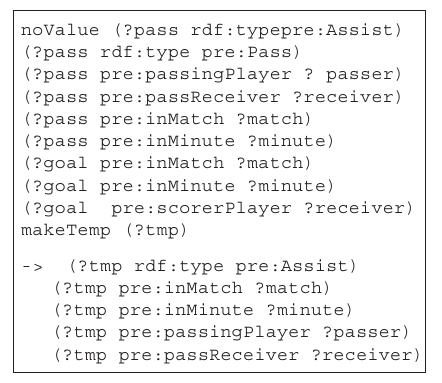
\includegraphics[width=3in]{fig/trans/fig6.png} 
	\caption[]{\xiaosihao Jena规则范例}
	\end{figure} 

推理是一个需要开销的过程,尤其当声明数量很大的时候。这个问题要被妥善地解决才能保证系统的可扩展性。因此,为了解决这个问题,我们采取了一些措施。首先,我们保证每场球赛是彼此独立的,然后单独进行推理。然后,我们分离地把推理得到的信息加入到基础知识中云。所以,推理球赛所需的时间就与球赛的数量无关。第二,所以的推理任务,包括分类和推理,都是线下完成的,也就是优先查询。这样一来,因为在运行的同时不会有线上推理,就可以提供可扩展性和查询效率。

3.6语义索引和检索

要查询一个语义性的基础知识并检索结果有很多方法。这些方法被分为四大类,基于关键词的,基于自然语言的,基于视觉的,基于形式的语义性搜索。在这些方法中,基于关键词的接口为末端用户提供了最轻松舒适的查询方法。对于其他方法,尽管他们可以实现更为精确的查询,但是需要更多的依赖于领域大小的用户交互。尽管基于关键词的接口,有着歧义等缺点,但是也存在一些方法可以缩小这一点,我们在第6部分将会有阐述。现在,已经决定了用基于关键词查询,下一个问题就是怎样才能实现好的检索性能和可扩展性。答案很简单,采用语义性索引。

正如我们之前文献调研所提到的那样,现在的关键词方法要么在大体积的{\Times RDF}文件中进行实时的遍历,要么只是用了简单的{\Times RDF}三元组关系。换句话说,他们没有同时考虑到可扩展性和检索性能。我们提出了一个叫语义索引的模型,它继承了传统关键词搜索,并用领域本体进行信息抽取和推理。这种索引机制是基于{\Times Lucene}的,这是一个可扩展的性能优异的索引器和搜索器。通过继承{\Times Lucene}索引的定制排序,含有本体信息的文本就有更高的权值,这样一来就实现了语义性检索。索引结构和排序的细节将在3.6.1和3.6.2部分分别详述。

3.6.1索引结构

语义索引的结构在检索性能上起着至关重要的作用,我们建立了一个{\Times Lucene}索引,每一个条目代表一个足球事件。正如我们在上一部分所说的那样,每一个事件都有与之相联系的属性,比如主体和客体。信息也被包含在了各个事件中。我们在索引中也包括了与事件相关的文本解说。如果一个是事件是未知事件(一个没有被信息抽取机识别的事件),这一点将非常重要。把全文解说加入到索引中,可以容忍事件信息的不完整性,因此可以保证在传统全文搜索中的查全率。索引结构及例子在表一中可见。


	\begin{table}[htbp] 
	\centering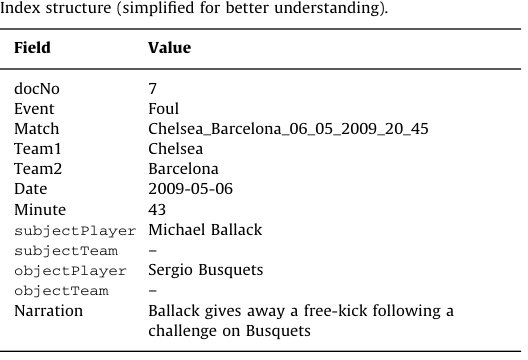
\includegraphics[width=3in]{fig/trans/tab1.png} 
	\caption[]{索引结构(为了便于理解简化)}
	\end{table} 

对于推理{\Times OWL}文件,我们建立了索引的扩展版,补充了索引中包含的基本信息,推理之后的索引也包含了事件的推理类型域,一个推理队员属性域和一个根据语义规则推理出的信息域。这些增加的信息都被加入到了推理索中,见表2 。注意主队和客队域也是用语义规则推理出来的。

	\begin{table}[htbp] 
	\centering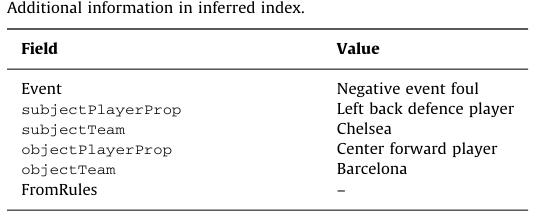
\includegraphics[width=3in]{fig/trans/tab2.png} 
	\caption[]{推理索引的补充信息}
	\end{table} 
3.6.2搜索和排序

在传统的关键词搜索中,索引文档通常除了一些与文档有关的粗糙的文本就什么有没有了。{\Times Lucene}能够轻松地控制索引,而且其默认排序就能给出很好的结果。然而,针对复杂的索引就要谨慎对待了。为了利用好我们面向索引结构的本体,我们稍微地修改了{\Times Lucene}中默认查询和排序机制。首先,我们扩大了排序域,包含了解析和推理的信息,以此强调他们的重要性。第二,这些域根据他们各自的重要性进行排序。例如,事件域就给了最高的排序顺位。这种方法可以避免文本中的一些歧义词误导或阴挡。例如,假设一个解说包含了“罗纳尔多错过了得分”。用传统的方法搜索进球的话,就会在第一位显示这个文档,而这恰恰是不好的假消息。然后,在针对本体的索引中,类型为得分的事件会有高排序顺位。因为上述事件的类型是错过,它只有较低的顺位。

4.评估

为了评估我们检索系统的检索性能,我们用爬虫搜索到了十场比赛,包含了一共1182条解说。在这些解说中,我们的IE模块能够解析其中的902个。用这些数据,我们为细节比较建立了四个{\Times Lucene}索引。首先,我们建立了一个传统的全文索引,{\Times TRAD},只用了{\Times UEFA}比赛的解说。这个索引是用来作为其他方法性能的基线。然后,我们建立了两个针对本体语义搜索的索引,{\Times BASIC\_EXT}和 {\Times FULL\_EXT},前者只包含了{\Times UEFA}的基本信息,而后者多了解析出来的信息。最后,我们建立了一个索引,{\Times FULL\_INF},它是{\Times FULL\_EXT}的扩展版,包含了推理出来的知识。所以的索引都用表3的查询来进行评估。
	\begin{table}[htbp] 
	\centering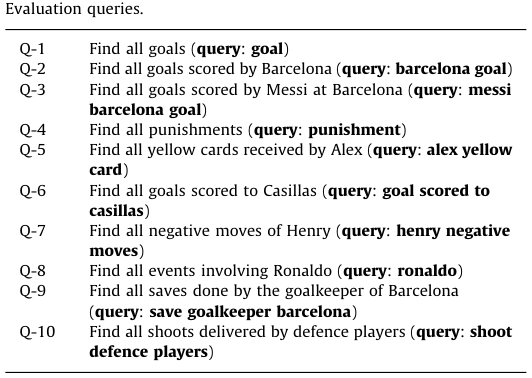
\includegraphics[width=3in]{fig/trans/tab3.png} 
	\caption[]{评价查询}
	\end{table} 

结果可以在表4中看到。首先,考虑前三个查询,{\Times TRAD}与其他方法就有了显著的区别。原因在于UEFA的解说中当{\Times P}得分了就用了短语“{\Times P}进了”。因为他省略了分这个字,在传统的索引中用关键词“得分”就不能检索出所有的进球。然而,信息解析模块能够成功地识别出进球,我们可以像文档那样在事件类型中给他填充为得分。因此,改善的索引就能响应“得分”和“进”这两种查询。这就是为什么{\Times BASIC\_EXT}和其他索引有非常高的查准率。
	\begin{table}[htbp] 
	\centering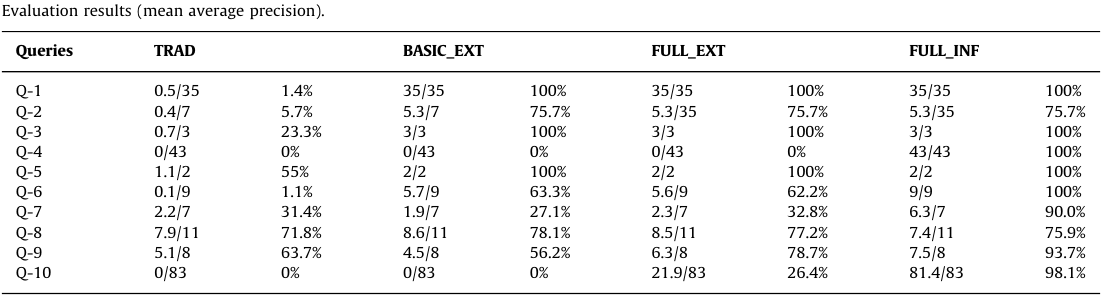
\includegraphics[width=6in]{fig/trans/tab4.png} 
	\caption[]{评价结果(平均查准率)}
	\end{table} 

这种能过信息解析模块产生的提高,可以通过{\Times BASIC\_EXT}和{\Times FULL\_EXT}中第9个和第10个的区别很容易看出来。这种区别源于解析射门和守门员扑救等事件。

这种提高源于推理,从查询4,7,10中很容易可以观察到。在这些查询中,{\Times FULL\_INF}索引表现得就比其他索引都要好,因为它包含了源于本体推理和分类的补充信息。例如,第4个查询提示了关于红牌和黄牌都是一种惩罚的推理知识。相似地,第10个查询则得益于通过分类推断出防守队员。最后,第7个查询用了定义于本体中的属性树的知识。这就意味着,系统可以识别属性,比如错过得分,越位和红牌,消极移动等。此外,在第6个查询中,我们可以看到{\Times Jena}规则的效果。在这儿,根据我们定义的规则之一,我们可以推断出精确的知识,比如哪次射门时是谁在守门,甚至并没有明确存在的知识。

如果我们看看查询8,就能发现四个索引效果并不多。原因在于,这是一个用单独的球员名字进行的简单搜索。所以,它并不包含太多语义索引可以利用的信息。然而,即使在这样的查询中,其性能也没有低于传统方法,因为全文的解说并没有被丢弃,而是保存在了一个独立的域中。换句话说,我们的方法保证了在最坏的情况下,也能与传统搜索一样。

我们的评估显示从{\Times BASIC\_EXT}开始,每一种索引都比它的前者有着显著的提高,而且最后在{\Times FULL\_INF}中,我们也达到了预期的效果。{\Times BASIC\_EXT}和{\Times FULL} {\Times \_EXT} 的性能也是让人满意的。在{\Times TRAD}和{\Times BASIC\_EXT}这间有明显的差别,因为它表现出即使是爬虫数据提供的基本信息,也会产生很大的不同。然而,当查询越来越复杂,我们需要具体的领域信息解析规则和推理来控制他们。所以,用这个框架,我们给开发者提供这样的机会,使他们可以根据用户的需要定制他们的系统。在任何情况下,这种框架都保证了提供可扩展性和用户友好性。

5.与查询扩展的比较

在第4部分,我们比较了我们的解决方法和传统方法,并看到了明显的提示不。然而,有人可能会问会不会出现这样的情况,只用扩展查询的方法就能达到之前的结果。因此,最后一个实验就展示了我们的解决方法和扩展查询方法的差异。为了填补这项空白,我们给用领域术语建的查询实现了一种原型,以此来扩展查询。例如,一个查询包含了“进球”将会扩展出动词“得分”,“错失”和其他派生词。本体信息也将被用在查询扩展中,因此,一个惩罚的查询将会被扩展到它的子类,比如“黄牌”“红牌”和动词“出牌”及其派生词。扩展查询直接在自由文本中运行,所以我们能清楚地看到查询扩展的提高,并能与我们的解决方案进行比较。

实验结果如表5所示。只要看一下,我们就能轻易地发现扩展查询的性能介于传统方法和语义索引,恰如我们所预料的那样。通过看查询1、2、3、4,我们能看到扩展查询的效果。前三个查询因为有了“得分”这个扩展,结果得以改善。在查询4中,因为有了惩罚这个术语的本体扩展,查询结果有了显著的提升。但是,性能依旧不如我们的本体索引法。因为没有合适的扩展术语,其他的查询结果没有受太大影响。对于一些搜索,这种搜索甚至会让结果更糟,因为它并不能正确捕捉到查询词汇的确切语义。
	\begin{table}[htbp] 
	\centering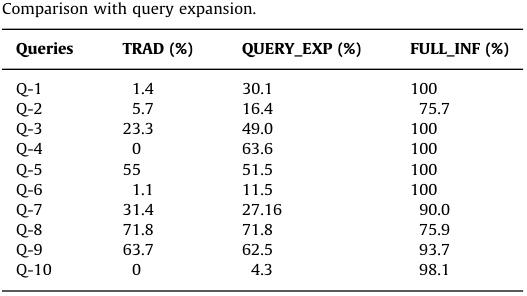
\includegraphics[width=3in]{fig/trans/tab5.png} 
	\caption[]{与查询扩展的比较}
	\end{table} 

6.增加短语支持

我们在3.6中提到了,关键词接口的搜索中最重要的问题是解决歧义。歧义出现通常有两种情况:词汇性的和结构性的。词汇性歧义由同义词导致,而结构性歧义由一词多义导致。只有信息扩展模块能够识别出词汇的歧义,我们才能解决,而我们并不没有实现一种词汇消除歧义的方法。然而,结构性歧义在关键词索引阶段就可以被解决。为了证明这一点,我们通过在现有系统上增加短语表达支持就解决了简单的结构性歧义问题。

假设一个用户想要查询{\Times Alex}对{\Times Ronaldo}的犯规,他会输入一个查询”犯规 {\Times Alex Ronaldo}”。系统可能会检索出{\Times Ronaldo}对{\Times Alex}的犯规,因为两个对员都可能犯规。为了解决这种结构性的歧义,我们引入了一些简单的短语表达,比如“对某人”,“被某人”,“属于某人”等,这样一来,系统就能知识查询对象是主体还是客体。这种实现的开销是微不足道的,因为只要填加了两个域,一个给主语,一个给宾语就可以实现了。每一个域的内容,都会有相应的介词与主语或是宾语相连。

我们对原始的版本({\Times FULL\_INF})和新的索引({\Times PHR\_EXP})做了比较。为此,我们做了三个人工查询。第一个查询测量主语混淆的性能({\Times Daniel}是制造犯规的人)。第二个查询往第一个中增加一个宾语({\Times Florent}),最后在第三种查询中,调换主宾的位置。结果见表6。注意到原来的索引在把握歧义的问题上遇到了困难,它并不能识别出谁是动作的主语,谁是宾语,但却不知道什么原因的,一直把{\Times Florent}当成了动作的主语。从另一方面来说,新的索引在任何条件下都能区分主语和宾语。
	\begin{table}[htbp] 
	\centering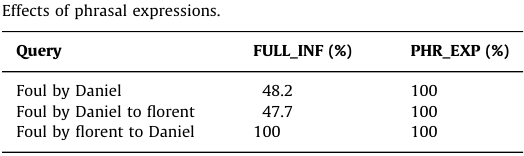
\includegraphics[width=3in]{fig/trans/tab6.png} 
	\caption[]{短语表达的影响}
	\end{table} 

7.讨论

本文展示了怎么样在保证了可扩展性和用户友好性的前提下,达到语义查询效果的。我们的方法还有另一个优势,那就是灵活性,尽管我们在研究中没有含盖,也就是说系统能够很容易的升级数据或是作出修改。我们认为用语义索引作为本体的上层,能够让基础知识变得更加灵活。

今天,大多数的语义应用都是以本体作为系统的主要数据结构,也就是说,要对本体的实例直接进行繁重的读写操作。然后,本体和本体实例都不是被用在这样的条件下的。从定义来看,他们是很严格的,是知识和声明的一种正式的代表。换言之,它们是永恒的,并不能这么随便改变更新。因此对于这些任务,我们推荐用另一种存储数据的方式,比如我们方案所用到的语义索引。

为了证明语义索引的灵活性,我们给出下面这个例子。假设我们想在查询接口中增加其他的语言,这样我们就能用两种语言来查询基础知识了。为了用本体实例达到这个目的,就必须要给第二语言复制实例和带有转换值的属性。在本体很庞大的时候,任何一种方案都是不实际的。但是,通过语义索引,要给每个域增加翻译过的值就非常容易。用语义网同义词,自然语言短语,甚至是词干来扩展索引的术语,都能被证明用语义索引是很容易就实现的。

8.结论和未来的工作

我们提出了一种新颖的语义检索框架,并应用足球领域,它含盖了语义网的各个方面,包括本体发展,信息抽取,本体构建,推理,语义规则,语义索引和检索。当这些技术被整合在关键词搜索的界面中,我们就获得了一种友好的,高性能的,可扩展的语义检索系统。评估结果显示,我们的方法超过了扩展查询或是传统的方法。此外,我们注意到我们的系统不用{\Times SPARQL}这样的正式的查询语句就可以实现复杂的语义性搜索。

我们注意到系统性能可于{\Times SPARQL}相媲美,而它恰是语义性搜索的最佳工具。最后,我们展示如何用语义索引来解决歧义的问题。

现在的工作可以在多方面进行扩展和改善。首先,我们准备丰富基础知识,来实现第7部分所提到的多语言支持。通过引入消除一词多义模块,我们的性能也会有很大提升。最后,我们未来的目标这一就是要设计这样一种机制,能根据用户反馈自动地扩展索引。



\vspace{20pt}
\centering 书面翻译对应的原文索引
\vspace{9pt}

\noindent
{\Times \wuhao \setlength{\baselineskip}{17pt}
Kara, S., Alan, Ö., Sabuncu, O., Akpınar, S., Cicekli, N. K., \& Alpaslan, F. N. (2012). An ontology-based retrieval system using semantic indexing. Information Systems, 37(4), 294-305.
}
